\subsection{Numerical Solution}\label{numericalSolution}

\par When using COMSOL Multiphysics to solve a two dimensional heat transfer PDE the user of the software must define the boundary conditions of the problem and specify the flux at each of those boundary conditions. This process is relatively similar to the analytical method described in Section \ref{numericalPDE}. The processes deviates when the user must specify the computational mesh element size and the geometry of the mesh showed in Figure \ref{fig:discreteSolution}. It should be noted that all computations performed in the thesis have access to the same computing resources described in Section \ref{resources}.

\begin{figure}[h]
\centering\fbox{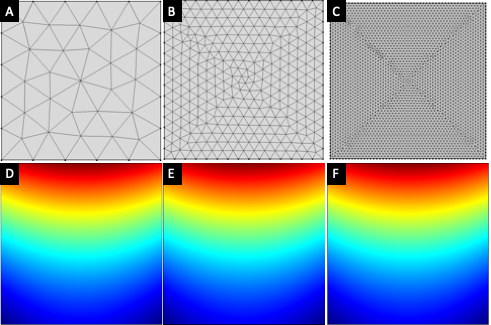
\includegraphics[height=3in,width=4.5in]{figures/figures2/01_discrete_pde.png}}
\caption{The finalized COMSOL geometry has one domain, 4 boundaries, and 4 vertices. \textbf{(A)} The physics controlled normal element size mesh consists of 68 domain elements and 20 boundary elements, \textbf{(B)} 578 domain elements and 60 boundary elements, and  \textbf{(C)} 6282 domain elements and 200 boundary elements. The number of degrees of freedom solved for is \textbf{(D)} 157 plus 44 internal DOFs and the solution is solved for in 1 seconds, \textbf{(E)} DOFs 1217 plus 124 internal DOFs solved for in 2 seconds, and \textbf{(F)} DOFs 12765 plus 404 internal DOFs solved for in 1 second.}
\label{fig:discreteSolution}
\end{figure}

\par The COMSOL Multiphyics numerical heat transfer PDE solutions are used to benchmark the accuracy of the analog algorithm implementations described in Section \ref{electricalPDE}, Section \ref{photonicPDE}, and Section \ref{metatronicPDE} because all 4 solutions include discretization error, described in Section \ref{discretizationError}, that deviates from the continuous analytical solution in Section \ref{analyticalPDE}. When striving to showcase the advantages of the analog algorithms, it is important to consider that the numerical solution benefits from the advantage of optimization of mesh geometry, shown in Figure \ref{fig:discreteSolution}, whereas the analog implementations have fixed rectangular meshes. The general lack of flexibility of analog implementations is one of there primary weaknesses, and what I try to compensate through reconfigurability.


\subsection{Discretization Error}\label{discretizationError}

\par In applied mathematics, discretization is the process of transferring continuous functions, models, variables, and equations into discrete counterparts. The discretization error is the error resulting from the fact that a function of a continuous variable is represented by a finite number of evaluations, in this case on a lattice. This visualization code for the discretization of our non physical analytical solution through the use of mesh scaling along a power law with exponent of 2 can found at \href{https://github.com/openhpclgw/roc_discrete_visualization.git}{\acrshort{roc} discrete visualization}. The discretization scaling is shown in figure \ref{fig:discrete}.

\par Discretization error is the principal source of error in the finite difference method employed in all of the information processing techniques this paper discusses. For a one dimensional problem the discretization error of $\varphi\left(x\right)$ can be defined in terms of its derivative

\begin{equation}\label{eq:discretizationError1D}
  \varphi^{\prime}\left(x\right) = \lim _ { h \rightarrow 0 } \frac { f \left( x + h \right) - f \left( x \right) } { h } \approx \frac { f \left( x + h \right) - f \left( x \right) } { h }
\end{equation}

where $h$ is finitely small and the removal of the limit creates the approximation which is defined as the discretization error. For a dense discretized solutions where the number of nodes $n$ approaches the limit $\left(2^n \Rightarrow 2^{\infty} \right)$ and acts like a continuous solution allows us to quantify the amount of inaccuracy generated by the discretization process and therefor better understand the effects of the physical properties of the electrical, optical, and metatronic information processing on their achievable accuracy's by accounting for inaccuracies caused by discretization which exists in all analog algorithm implementations.

\begin{figure}[h]
\centering\fbox{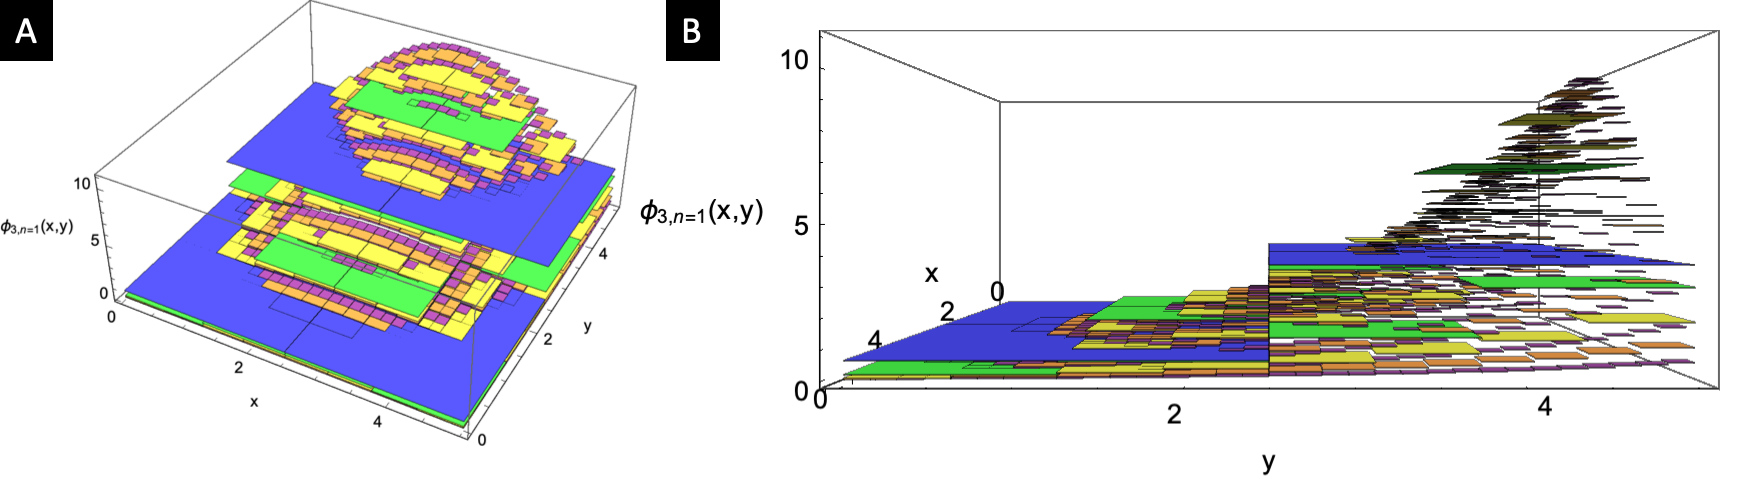
\includegraphics[height=1.5in,width=4.5in]{figures/figures2/02_discretization.png}}
\caption{\textbf{(A)} Plot of $\psi_{3,n}\left(x,y\right)$ with $L=5$ and $H=5$ with the the discretized mesh $2^1 = 2$ blue, $2^2 = 4$ green, $2^3 = 8$ yellow, $2^4 = 16$ orange, and $2^5 = 32$ purple solutions shown in the z axis. \textbf{(B)} The right side view is shown.}
\label{fig:discrete}
\end{figure}